\subsection{Visualisation}

With the files processed by Flink and stored on MongoDB, Hive and Cassandra we have built several workbooks on Tableau:

\begin{itemize}
	\item \textbf{Live Map}: A map of the world tracking all active flights in real time (Using either MongoDB or Cassandra as data source).
	\item \textbf{Inbound Flow}: Set of different charts to analyse the flow of flights directed towards an airport of choice (Using either MongoDB or Hive as data source).
	\item \textbf{Outbound Flow}: Set of different charts to analyse the flow of flights departing from an airport of choice (Using either MongoDB or Hive as data source).
	\item \textbf{Flight Route}: A route tracked on the map of the world showing the path followed by an aeroplane of choice (Using MongoDB as data source).
\end{itemize}
\subsubsection{Connection to Data Source}

In order to connect Tableau to a data source two middlewares are required: a \textbf{Connector}, to translate Tableau's own VizQL to the target database query language, and an \textbf{ODBC} in which to specify the address and port in which the database is to be found to do the actual connection.
\\
Tableau uses internally a relational model and VizQL is therefore a query language for such models; while for relational databases, such as Hive, the query translation is pretty straightforward, for NoSQL databases like MongoDB and Cassandra the conversion is done with an additional step in which a schema is produced to translate the Document based and Key/Value models into relational models.

\subsubsection{Live Map}
The live map is used to monitor and track in real time planes flying all over the world. Data for this view are collected from Cassandra's Active table or MongoDB's Active collection through a live connection; this connection allows us to refresh the map as soon as new data are available in the database.
\\
The two most important variables for the construction of such graphic are latitude and longitude, used by Tableau to draw a marker on the map. Such marker, by default, is a bullet point, but in order to add a new dimension to the view we added a custom marker showing a plane directed towards the actual direction the flight is headed to.
\\
As for interactivity from the view, it is possible to read other details of a single plane or to use one or more of several filters:
\begin{itemize}
	\item \textbf{Origin}: Airport whence the plane departed.
	\item \textbf{Destination}: Airport where the plane is headed towards.
	\item \textbf{Flight}: The unique code given to a flight.
	\item \textbf{Aircraft}: The aircraft's model's unique code.
\end{itemize}

Figure \ref{fig:LiveMap} shows a close up of the middle east without any filtering.
\begin{figure}[h]
	\centering
	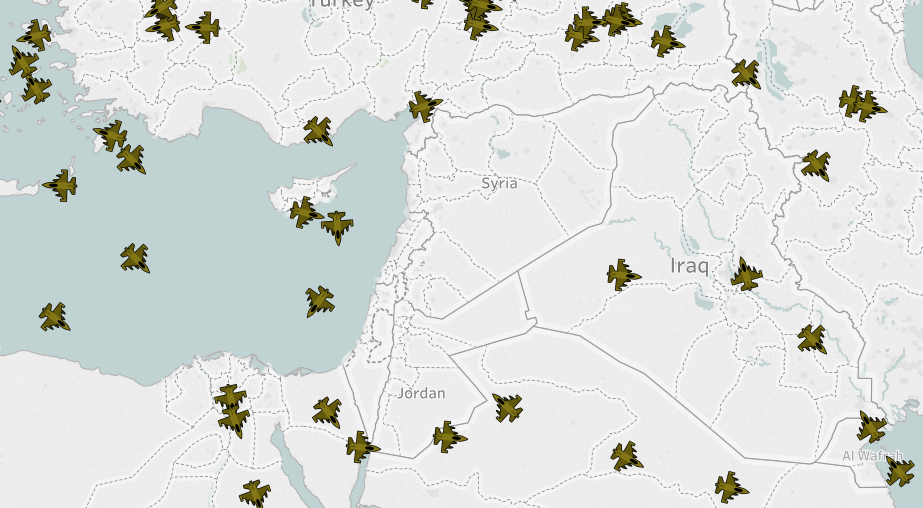
\includegraphics[width=0.9\linewidth]{Figures/LiveMap.png}
	\caption{A close up of the live map over the middle east}
	\label{fig:LiveMap}
\end{figure}

\subsubsection{Inbound Flow}

The second view built aims to present historical data of flights that have landed at an airport. For this kind of periodic analysis for which we have not need of real time connections, we have chosen to use the extract connection; this extract is updated each day and guarantees superior performances in charts' rendering.
\\
Before the extraction, we have set up a join between historical data and collections with information on aircrafts and airports in order to enrich the data source, furthermore fields not utilised in the presentation have been cleansed to lighten the load.
\\
Data are presented in three dashboards focusing on:

\begin{itemize}
	\item \textbf{Flights}: The total number of flights landed at an airport.
	\item \textbf{Aircraft}: The type of aircraft of those flights.
	\item \textbf{Passengers}: The total number of passengers landed at an airport.
\end{itemize}

Whatever the focus, the first useful operation is to filter by selecting an airport for which to analyse the flow. After that several temporal filters are available with complete control of the granularity of time through drill-down and drill-up. It is also possible to change type of chart from classical histogram to geographical maps and heat maps.

Figure \ref{fig:FlightsViz} shows a histogram depicting the flow of flights from the world towards Albuquerque in the month of November from 8 AM to 8 PM, day by day.

\begin{figure}[h]
	\centering
	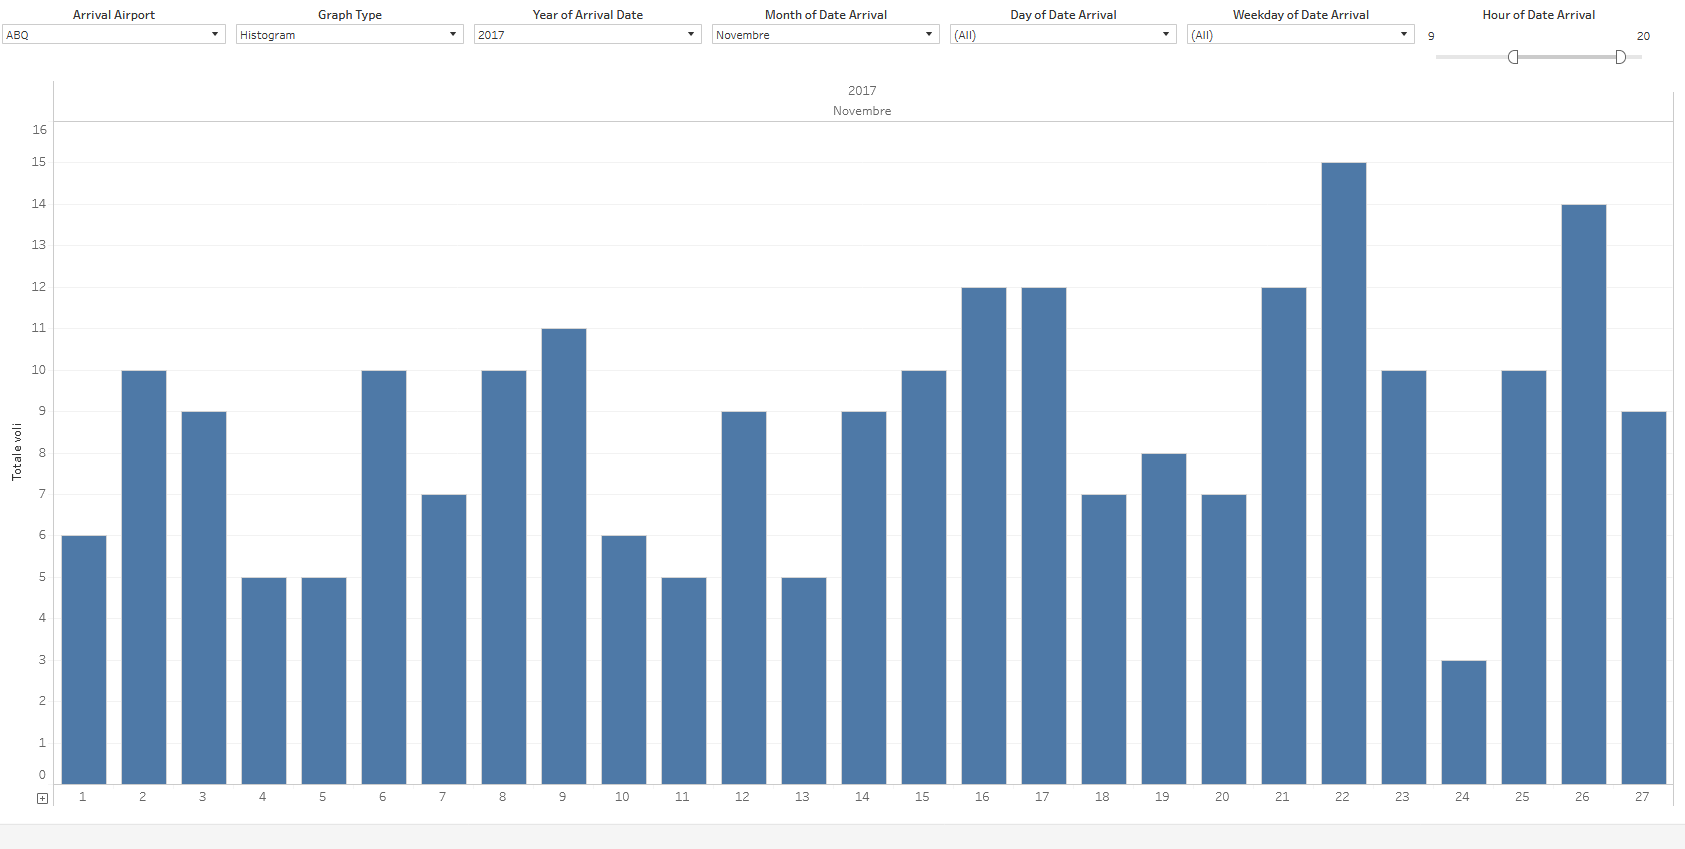
\includegraphics[width=0.9\linewidth]{Figures/FlightsViz.png}
	\caption{Inbound Flow for Albuquerque day by day 8 AM to 8 PM, November}
	\label{fig:FlightsViz}
\end{figure}

\subsubsection{Outbound Flow}
A carbon copy of the inbound flow has been realised to analyse the flow departing from an airport.\\
This duplication is done in order to optimise performances on both views. From an implementation point of view the only change is in the join condition to use during the extract creation and the use of the time of departure as timestamp, instead of the time of arrival.

Figure \ref{fig:PassengersViz} shows a map depicting the main destinations of the passengers departing from Genoa in October and November.

\begin{figure}[h]
	\centering
	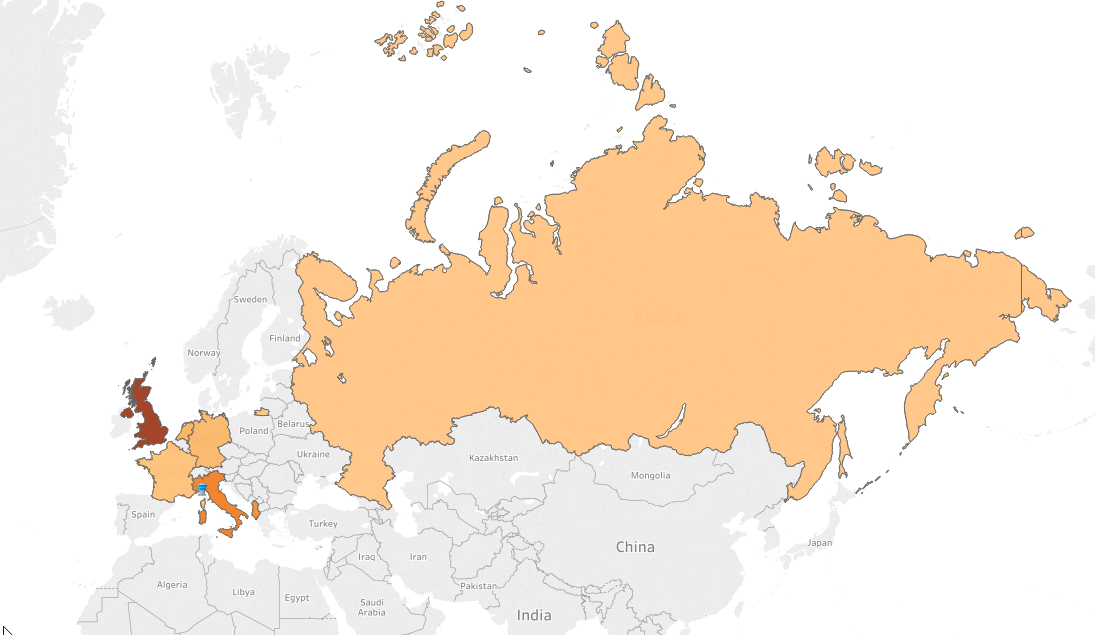
\includegraphics[width=0.9\linewidth]{Figures/PassengersViz.png}
	\caption{Outbound Flow of passengers for Genoa, October and November}
	\label{fig:PassengersViz}
\end{figure}

\subsubsection{Flight Route}
Given a flight code, it is possible to draw the path the aeroplane followed on each day for that route. This view shows the limits of Satori as an end-point, because we can only see messages coming from a height over 37000 feet, cutting the taking off and the landing parts of the fare.

 Figure \ref{fig:RouteViz} shows, through a set of points coming from consequent messages from the same plane, the route of flight UA914, from Paris to Washington, of October 25th; here it can be seen the filter cutting data below 37000 feet in action.
\begin{figure}[h]
	\centering
	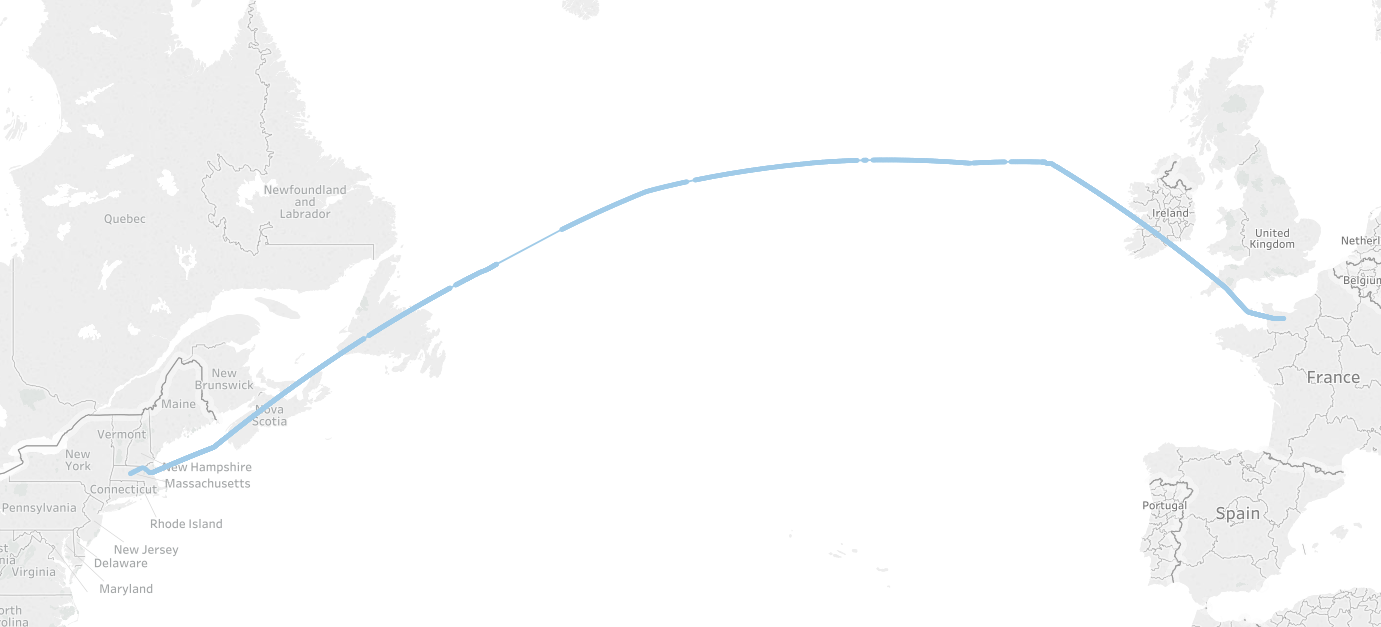
\includegraphics[width=0.9\linewidth]{Figures/RouteViz.png}
	\caption{The route of flight UA914, from Paris to Washington, of October 25th}
	\label{fig:RouteViz}
\end{figure}
This view is built with a live connection with the use of Custom SQL. Thanks to the definition of an ad hoc query, MongoDB's Raw collection is queried using the flight code as a parameter.
The query is then converted to an aggregation pipeline in MongoDB with a dedicated process, resulting in a response within few seconds, in spite of the huge size of the collection (more than a billion documents).
\subsubsection{Publishing on Tableau Server}
Once the workbooks have been created, we proceeded by publishing all the views on Tableau Server. For this purpose, we have defined two user groups with different rights: the Devs who inherit the powers and rights of the Publisher and can create, edit and interact with the workbooks; the Users which inherit the right of the Interactor and can, therefore, only interact with the workbooks.

In order to use the views freely, it had been necessary to save the required credentials for the authentication on the data sources directly on the Tableau workbook.
Finally, we have scheduled a daily update at 4 AM to refresh the extracts for the visualisations of historical data.